% Nội dung lấy từ slide môn học (ngày 03/11/2026)
% Hình trong IMAGE/slide/ cắt từ PDF slide ở docs/ bằng script, Hình thành phần DSS vẽ bằng TikZ
\section{Cơ sở lý thuyết}
\subsection{Kho dữ liệu}
\subsubsection{Định nghĩa}
Kho dữ liệu (Data Warehouse) là nơi lưu trữ thông tin tập trung, có thể đem ra phân tích để đưa ra quyết định tốt hơn. Dữ liệu trong kho được gom từ các hệ thống tác nghiệp và các nguồn khác. Sau đó dữ liệu được làm sạch, chuẩn hoá và sắp xếp lại cho việc phân tích. Hai tác giả thường được nhắc đến khi nói về kho dữ liệu là Inmon~\cite{inmon2005} và Kimball~\cite{kimball2013}.

\subsubsection{Các đặc trưng của kho dữ liệu}
Kho dữ liệu có bốn đặc trưng chính~\cite{inmon2005}:
\begin{itemize}
    \item \textbf{Hướng chủ đề (subject-oriented):} dữ liệu được tổ chức theo các chủ đề chính của doanh nghiệp như khách hàng, sản phẩm, doanh số. Nó không tổ chức theo từng ứng dụng tác nghiệp.
    \item \textbf{Tích hợp (integrated):} dữ liệu đến từ nhiều nguồn khác nhau nên phải được thống nhất. Ví dụ cùng một dữ liệu nhưng khác tên, khác dữ liệu nhưng trùng tên, hay mã hoá không đồng nhất như 0/1, m/f, male/female.
    \item \textbf{Không biến động (nonvolatile):} dữ liệu đã nạp vào kho thì không bị sửa liên tục như trong cơ sở dữ liệu tác nghiệp. Người dùng chủ yếu đọc dữ liệu.
    \item \textbf{Gắn với thời gian (time-variant):} kho lưu lịch sử. Mỗi giá trị gắn với một thời điểm, giống như các ảnh chụp (snapshot) liên tiếp nhau.
\end{itemize}

\subsubsection{Kiến trúc của kho dữ liệu}
Kiến trúc tổng quát của kho dữ liệu được thể hiện ở Hình~\ref{fig:kien_truc_dw}, lấy từ Elmasri và Navathe~\cite{elmasri2016}. Dữ liệu đi từ các cơ sở dữ liệu nguồn, qua bước ETL, rồi vào kho. Trong kho có hai phần là dữ liệu và siêu dữ liệu (metadata). Từ kho, dữ liệu được dùng cho các ứng dụng phân tích như OLAP, DSS, hệ thông tin điều hành (EIS) và khai phá dữ liệu.

\begin{figure}[!htbp]
\centering
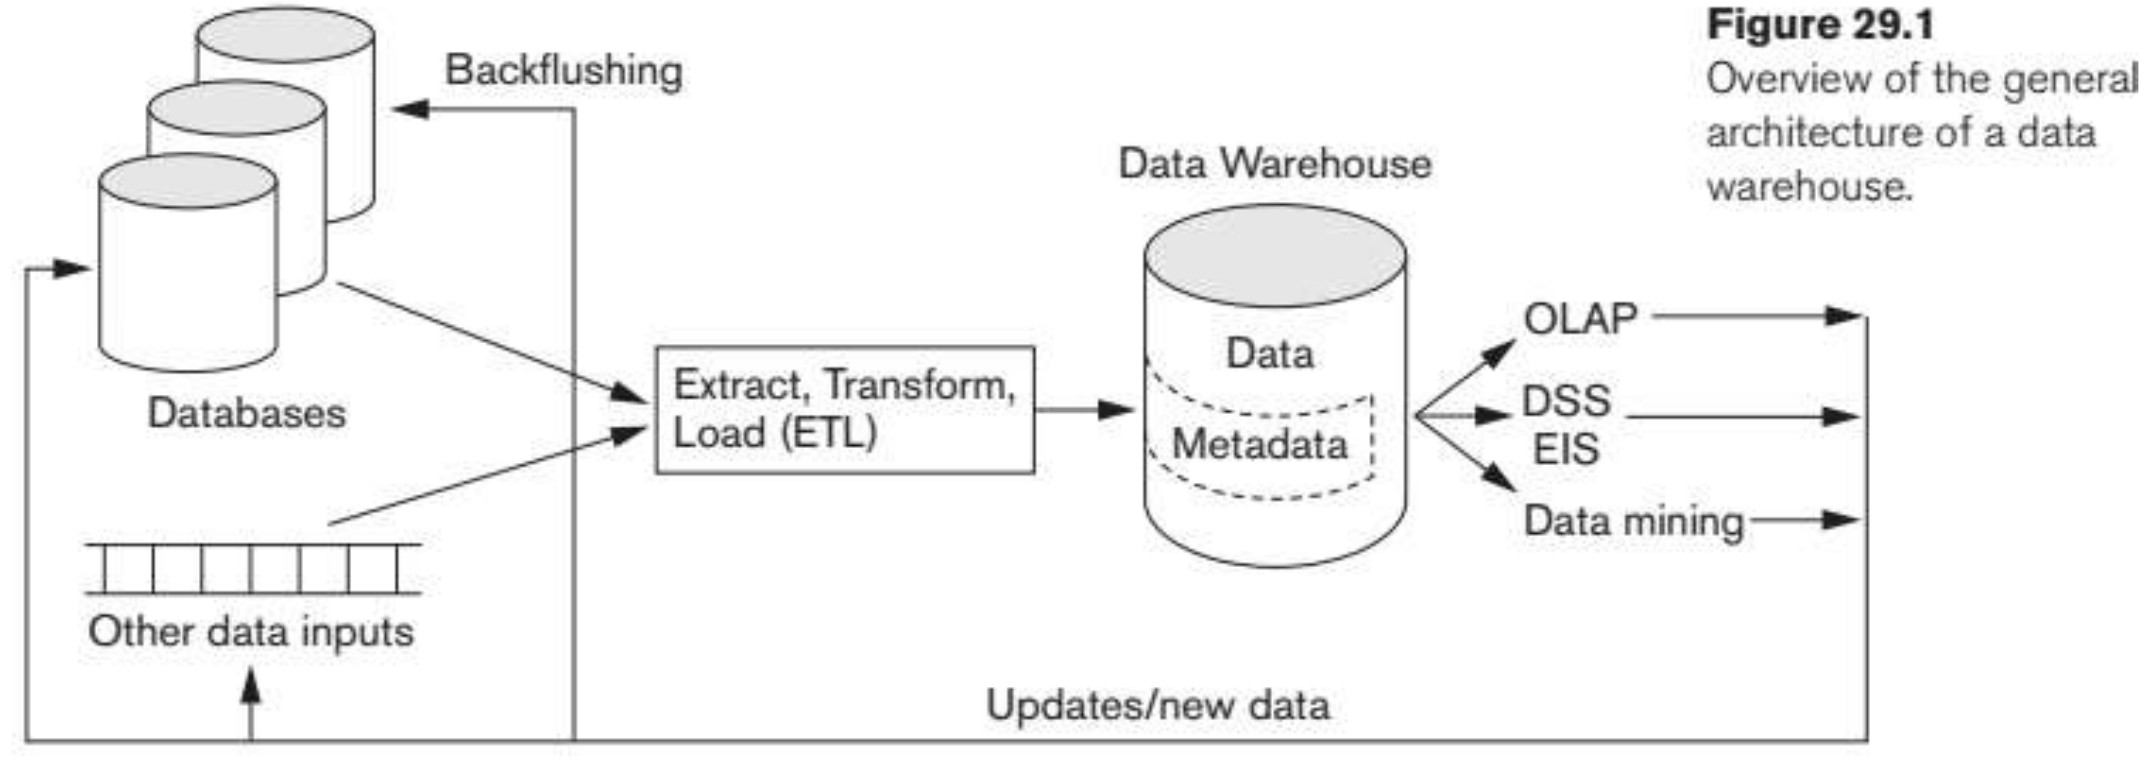
\includegraphics[width=0.9\textwidth]{slide/kien_truc_dw.png}
\caption{Kiến trúc tổng quát của kho dữ liệu}
\label{fig:kien_truc_dw}
\end{figure}

Kho dữ liệu khác hẳn cơ sở dữ liệu tác nghiệp (OLTP). OLTP phục vụ giao dịch hằng ngày, còn kho dữ liệu phục vụ phân tích (OLAP). Bảng~\ref{tab:oltp_olap} tóm tắt các điểm khác nhau chính~\cite{han2011}.

\begin{table}[!htbp]
\centering
\caption{So sánh hệ thống OLTP và OLAP}
\label{tab:oltp_olap}
\begin{tabular}{p{3.2cm}p{5cm}p{5.5cm}}
\toprule
\textbf{Tiêu chí} & \textbf{OLTP} & \textbf{OLAP} \\
\midrule
Định hướng & Giao dịch & Phân tích \\
Người dùng & Nhân viên nhập liệu, quản trị CSDL & Nhà quản lý, chuyên viên phân tích \\
Thiết kế CSDL & Mô hình ER, chuẩn hoá cao & Mô hình sao hoặc bông tuyết, phi chuẩn hoá \\
Dữ liệu & Hiện hành, chi tiết & Lịch sử, tổng hợp, đa chiều \\
Truy cập & Đọc và ghi & Chủ yếu là đọc \\
Đơn vị công việc & Giao dịch ngắn, đơn giản & Truy vấn phức tạp \\
\bottomrule
\end{tabular}
\end{table}

\subsection{Một số khái niệm khác}
\subsubsection{Mô hình hoá chiều}
Kimball đề xuất thiết kế kho bằng mô hình hoá chiều (dimensional modeling)~\cite{kimball2013}. Mô hình này có hai loại bảng. Bảng sự kiện (fact) chứa các số đo của nghiệp vụ, ví dụ số tiền bán, cùng các khoá ngoại trỏ tới bảng chiều. Bảng chiều (dimension) chứa các thuộc tính mô tả dùng để lọc và nhóm dữ liệu, ví dụ ngày, sản phẩm, khách hàng.

Khi bảng sự kiện nằm giữa và nối thẳng tới các bảng chiều, ta có mô hình sao (star schema). Nếu bảng chiều được tách nhỏ thêm theo cấp bậc, ta có mô hình bông tuyết (snowflake schema). Hình~\ref{fig:sao_bong_tuyet} so sánh hai mô hình này với cùng bảng sự kiện Sales Facts~\cite{empire}.

\begin{figure}[!htbp]
\centering
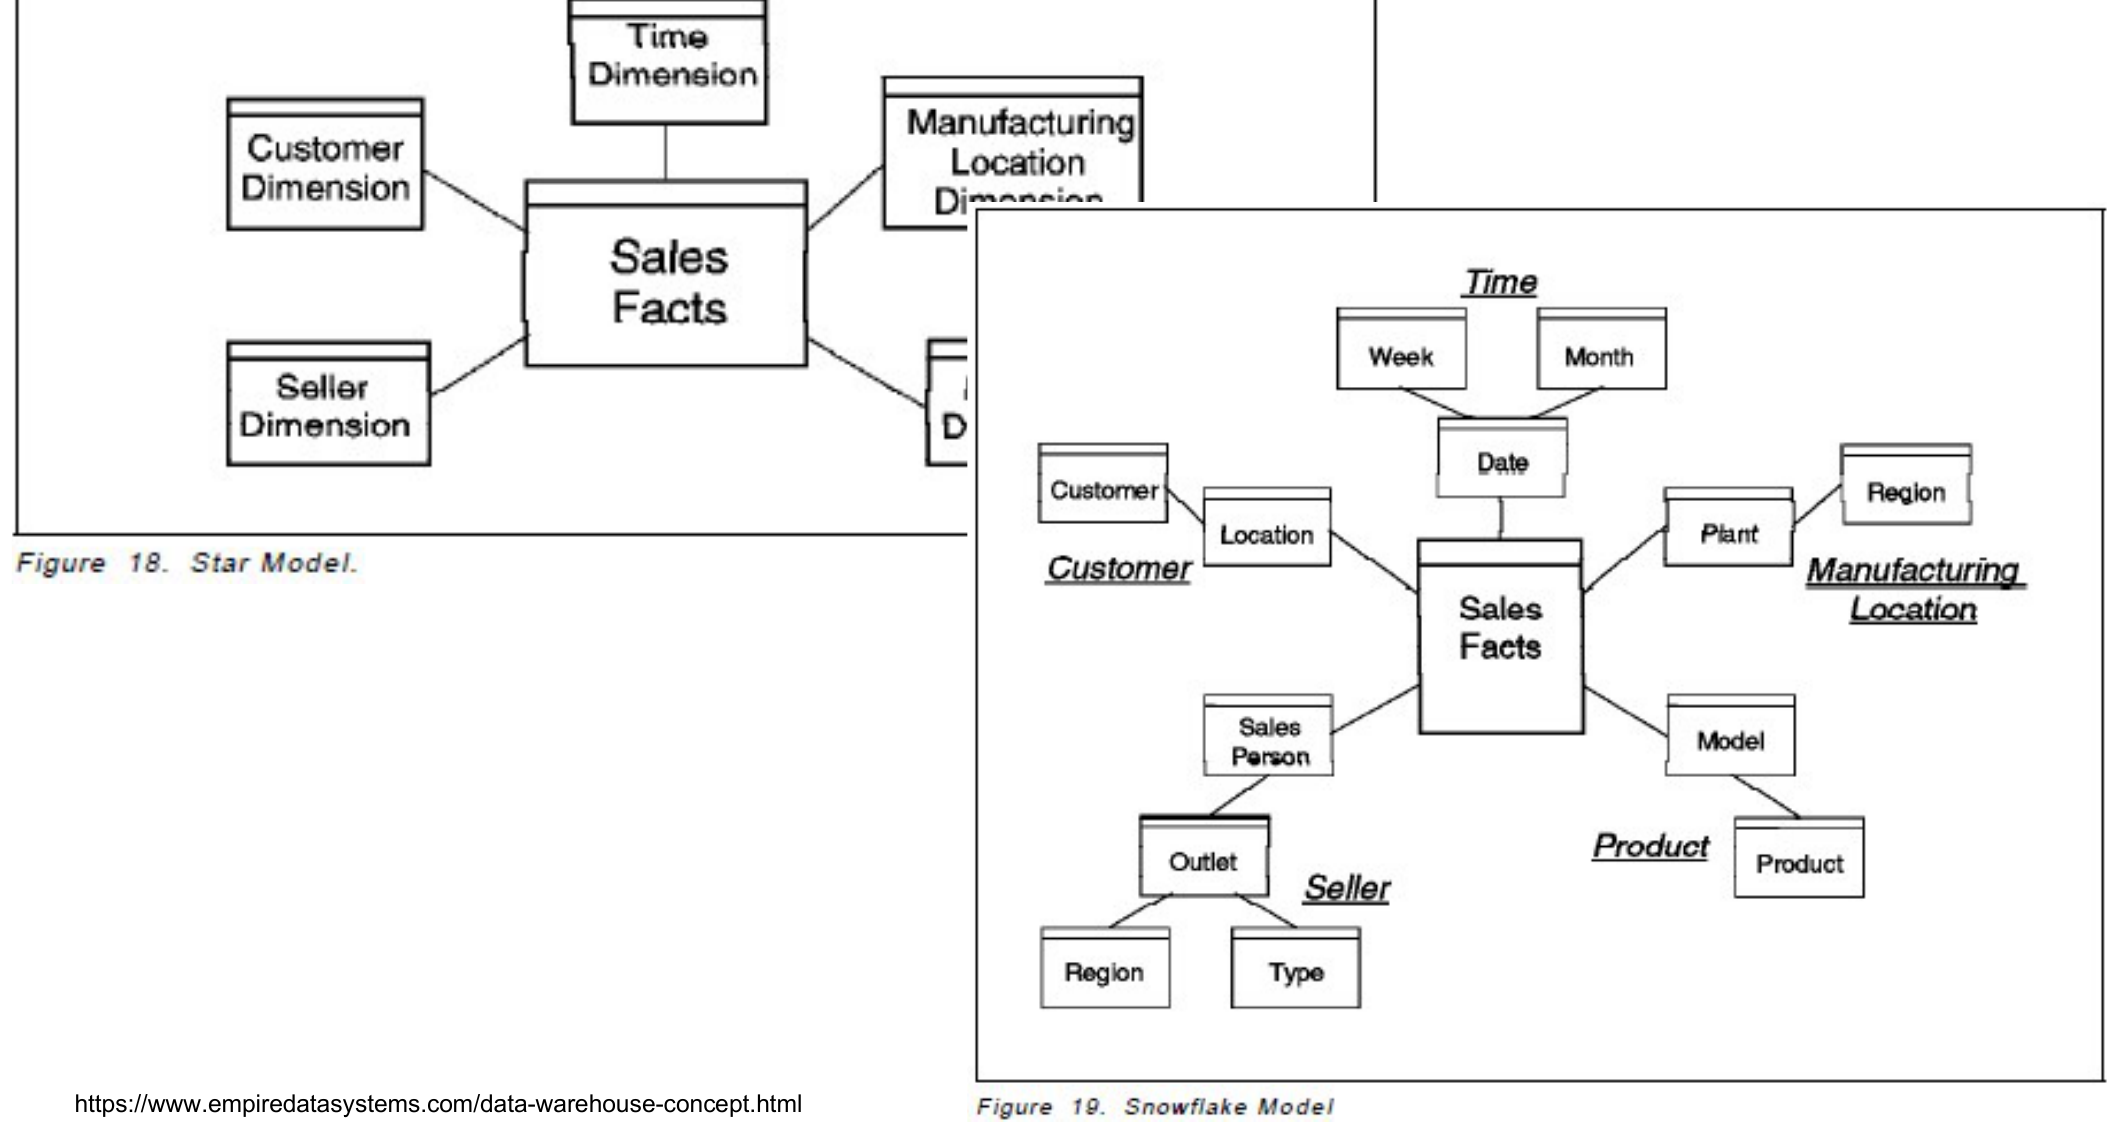
\includegraphics[width=0.95\textwidth]{slide/sao_bong_tuyet.png}
\caption{Mô hình sao (trái) và mô hình bông tuyết (phải)}
\label{fig:sao_bong_tuyet}
\end{figure}

Thiết kế theo mô hình chiều gồm bốn bước~\cite{kimball2013}. Đầu tiên là chọn quy trình nghiệp vụ. Tiếp theo là khai báo độ mịn (grain), tức là một dòng trong bảng sự kiện thể hiện điều gì. Sau đó xác định các chiều, và cuối cùng xác định các số đo. Khi thuộc tính của bảng chiều thay đổi theo thời gian, kho xử lý bằng các kiểu chiều thay đổi chậm (slowly changing dimension, SCD). Hai kiểu hay dùng là kiểu 1 ghi đè giá trị cũ, và kiểu 2 thêm dòng mới để giữ lịch sử.

\subsubsection{Quy trình ETL trong kho dữ liệu}
ETL gồm ba bước. Trích xuất (Extract) lấy dữ liệu từ các nguồn nội bộ và bên ngoài. Biến đổi (Transform) làm sạch, đổi định dạng và hợp nhất dữ liệu. Nạp (Load) đưa dữ liệu đã biến đổi vào kho. Một biến thể là ELT, trong đó dữ liệu thô được nạp vào kho trước rồi mới biến đổi.

Khó khăn chính của ETL nằm ở việc tích hợp dữ liệu. Các nguồn có thể đặt tên khác nhau cho cùng một dữ liệu, hoặc mã hoá khác nhau. Dữ liệu cũng có thể thiếu, sai hay không nhất quán. Vì vậy quy trình ETL phải kiểm tra chất lượng dữ liệu theo các tiêu chí như độ chính xác, độ đầy đủ, tính nhất quán và tính kịp thời.

\subsubsection{Quá trình phân tích đa chiều (OLAP)}
OLAP xem dữ liệu như một khối nhiều chiều (cube). Mỗi chiều là một trục, ví dụ thời gian, sản phẩm, khu vực. Mỗi ô trong khối chứa một số đo. Trên khối này có bốn phép thao tác cơ bản~\cite{han2011}:
\begin{itemize}
    \item \textbf{Roll-up:} gộp dữ liệu lên mức tổng quát hơn, ví dụ từ tháng lên quý.
    \item \textbf{Drill-down:} đi ngược lại, xuống mức chi tiết hơn, ví dụ từ chi nhánh xuống từng nhóm bán hàng.
    \item \textbf{Slice:} cố định giá trị của một chiều để lấy ra một lát cắt.
    \item \textbf{Dice:} đặt điều kiện trên hai chiều trở lên để lấy ra một khối con.
\end{itemize}
Hình~\ref{fig:olap} minh hoạ bốn phép này trên bảng số lượng bán theo sản phẩm, khu vực và thời gian~\cite{empire}. Theo cách lưu trữ, OLAP có ba loại: ROLAP lưu trên cơ sở dữ liệu quan hệ, MOLAP lưu trên khối đa chiều, và HOLAP kết hợp cả hai.

\begin{figure}[!htbp]
\centering
\begin{subfigure}[b]{0.40\textwidth}
    \centering
    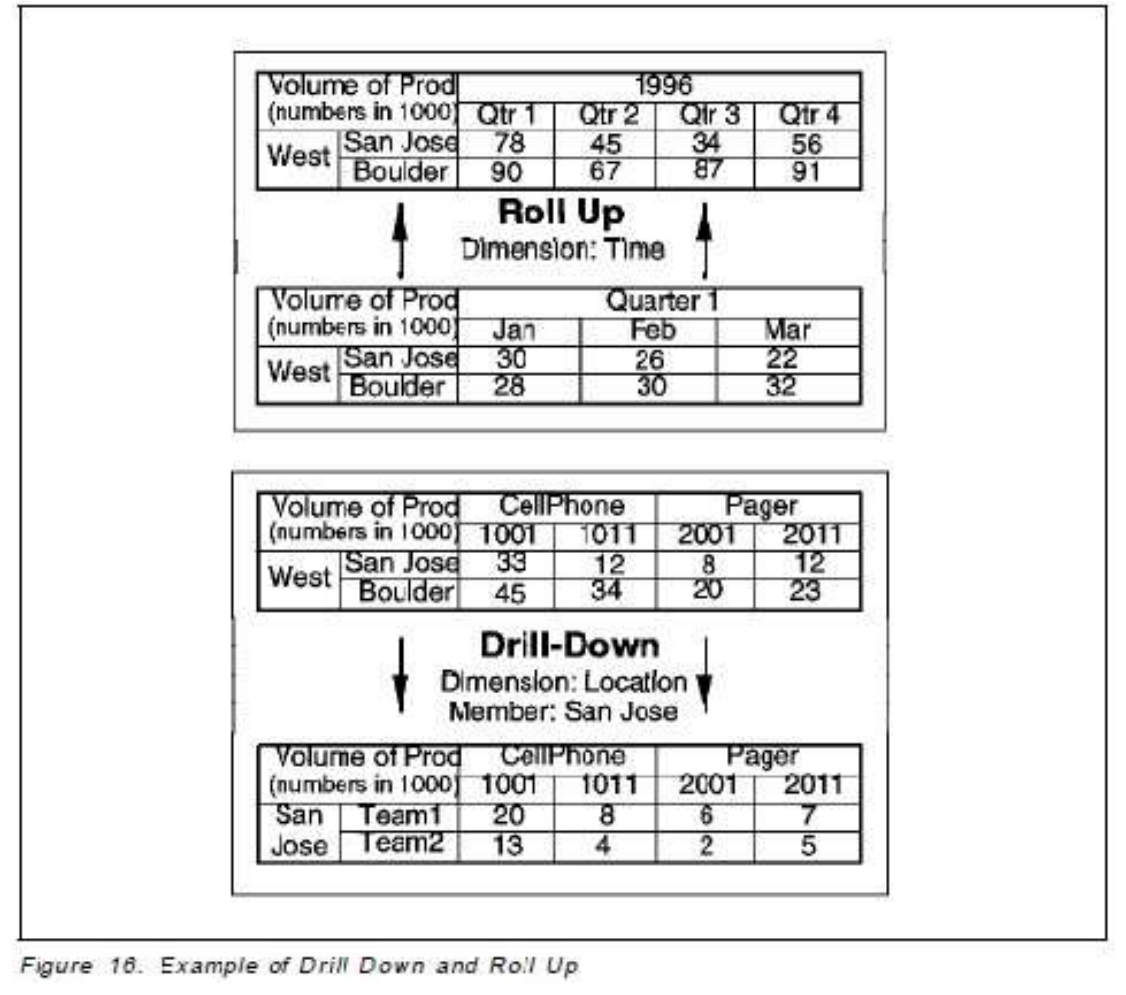
\includegraphics[width=\textwidth]{slide/rollup_drilldown.png}
    \caption{Roll-up và drill-down}
\end{subfigure}
\hfill
\begin{subfigure}[b]{0.56\textwidth}
    \centering
    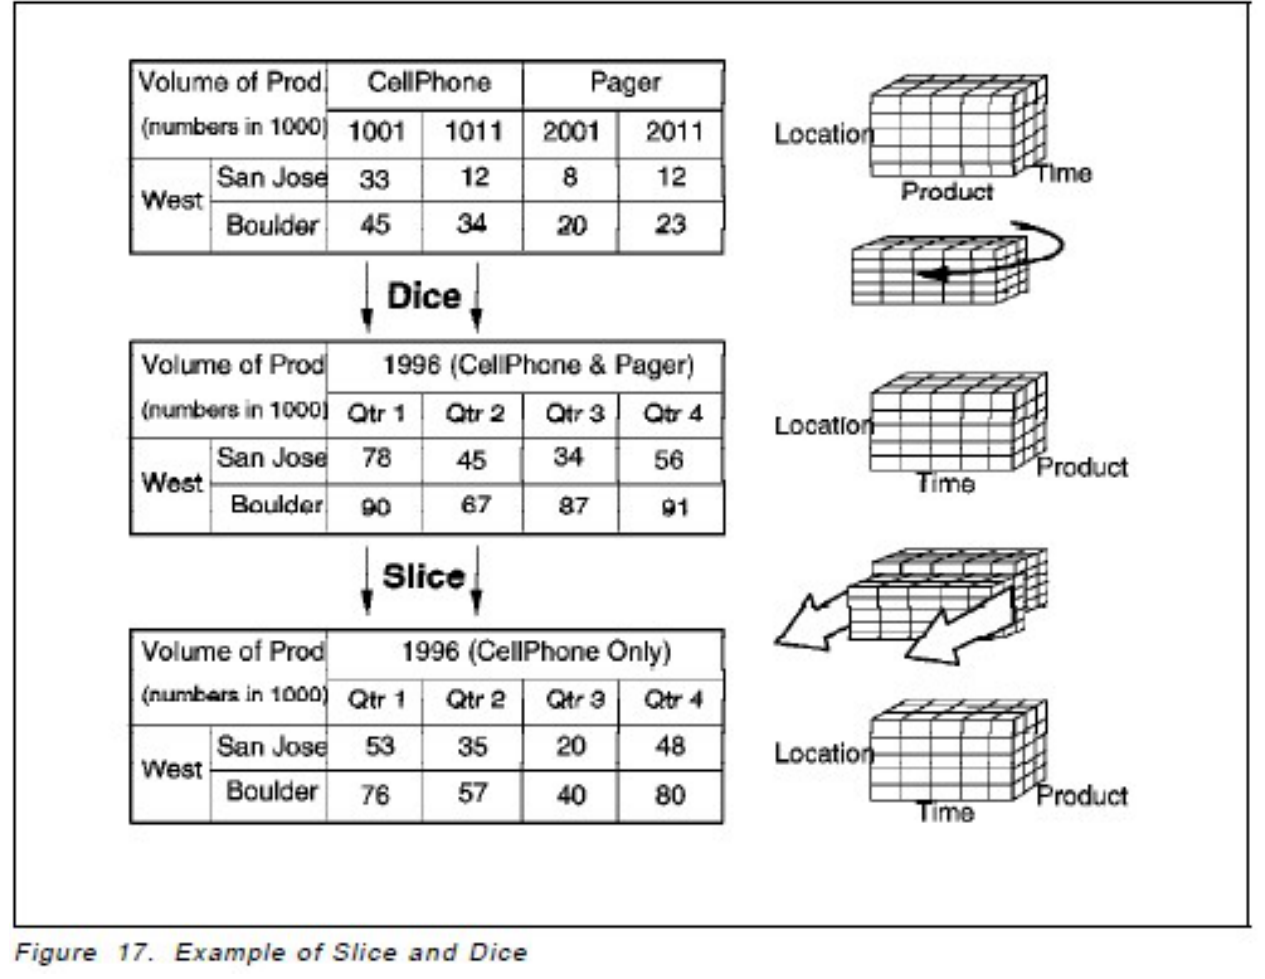
\includegraphics[width=\textwidth]{slide/slice_dice.png}
    \caption{Dice và slice}
\end{subfigure}
\caption{Các phép thao tác OLAP}
\label{fig:olap}
\end{figure}

\subsection{Hệ hỗ trợ ra quyết định}
\subsubsection{Định nghĩa và quá trình ra quyết định}
Hệ hỗ trợ ra quyết định (Decision Support System, DSS) là một loại hệ thống thông tin giúp hỗ trợ và cải thiện việc ra quyết định~\cite{turban2005}. DSS thuộc nhóm lớn hơn là hệ hỗ trợ quản lý (Management Support System, MSS). MSS là việc áp dụng công nghệ để hỗ trợ công việc quản lý, đặc biệt là ra quyết định.

Theo Simon, việc ra quyết định đi qua bốn pha~\cite{turban2005}, như Hình~\ref{fig:simon}. Pha nhận thức (intelligence) xem xét thực tế để phát hiện và phát biểu vấn đề. Pha thiết kế (design) xây dựng mô hình đại diện cho vấn đề, xác định các biến và quan hệ giữa chúng. Pha lựa chọn (choice) chọn ra một giải pháp từ mô hình. Pha thực hiện (implementation) đưa giải pháp vào thực tế. Kết quả thực hiện được theo dõi và phản hồi lại các pha trước.

\begin{figure}[!htbp]
\centering
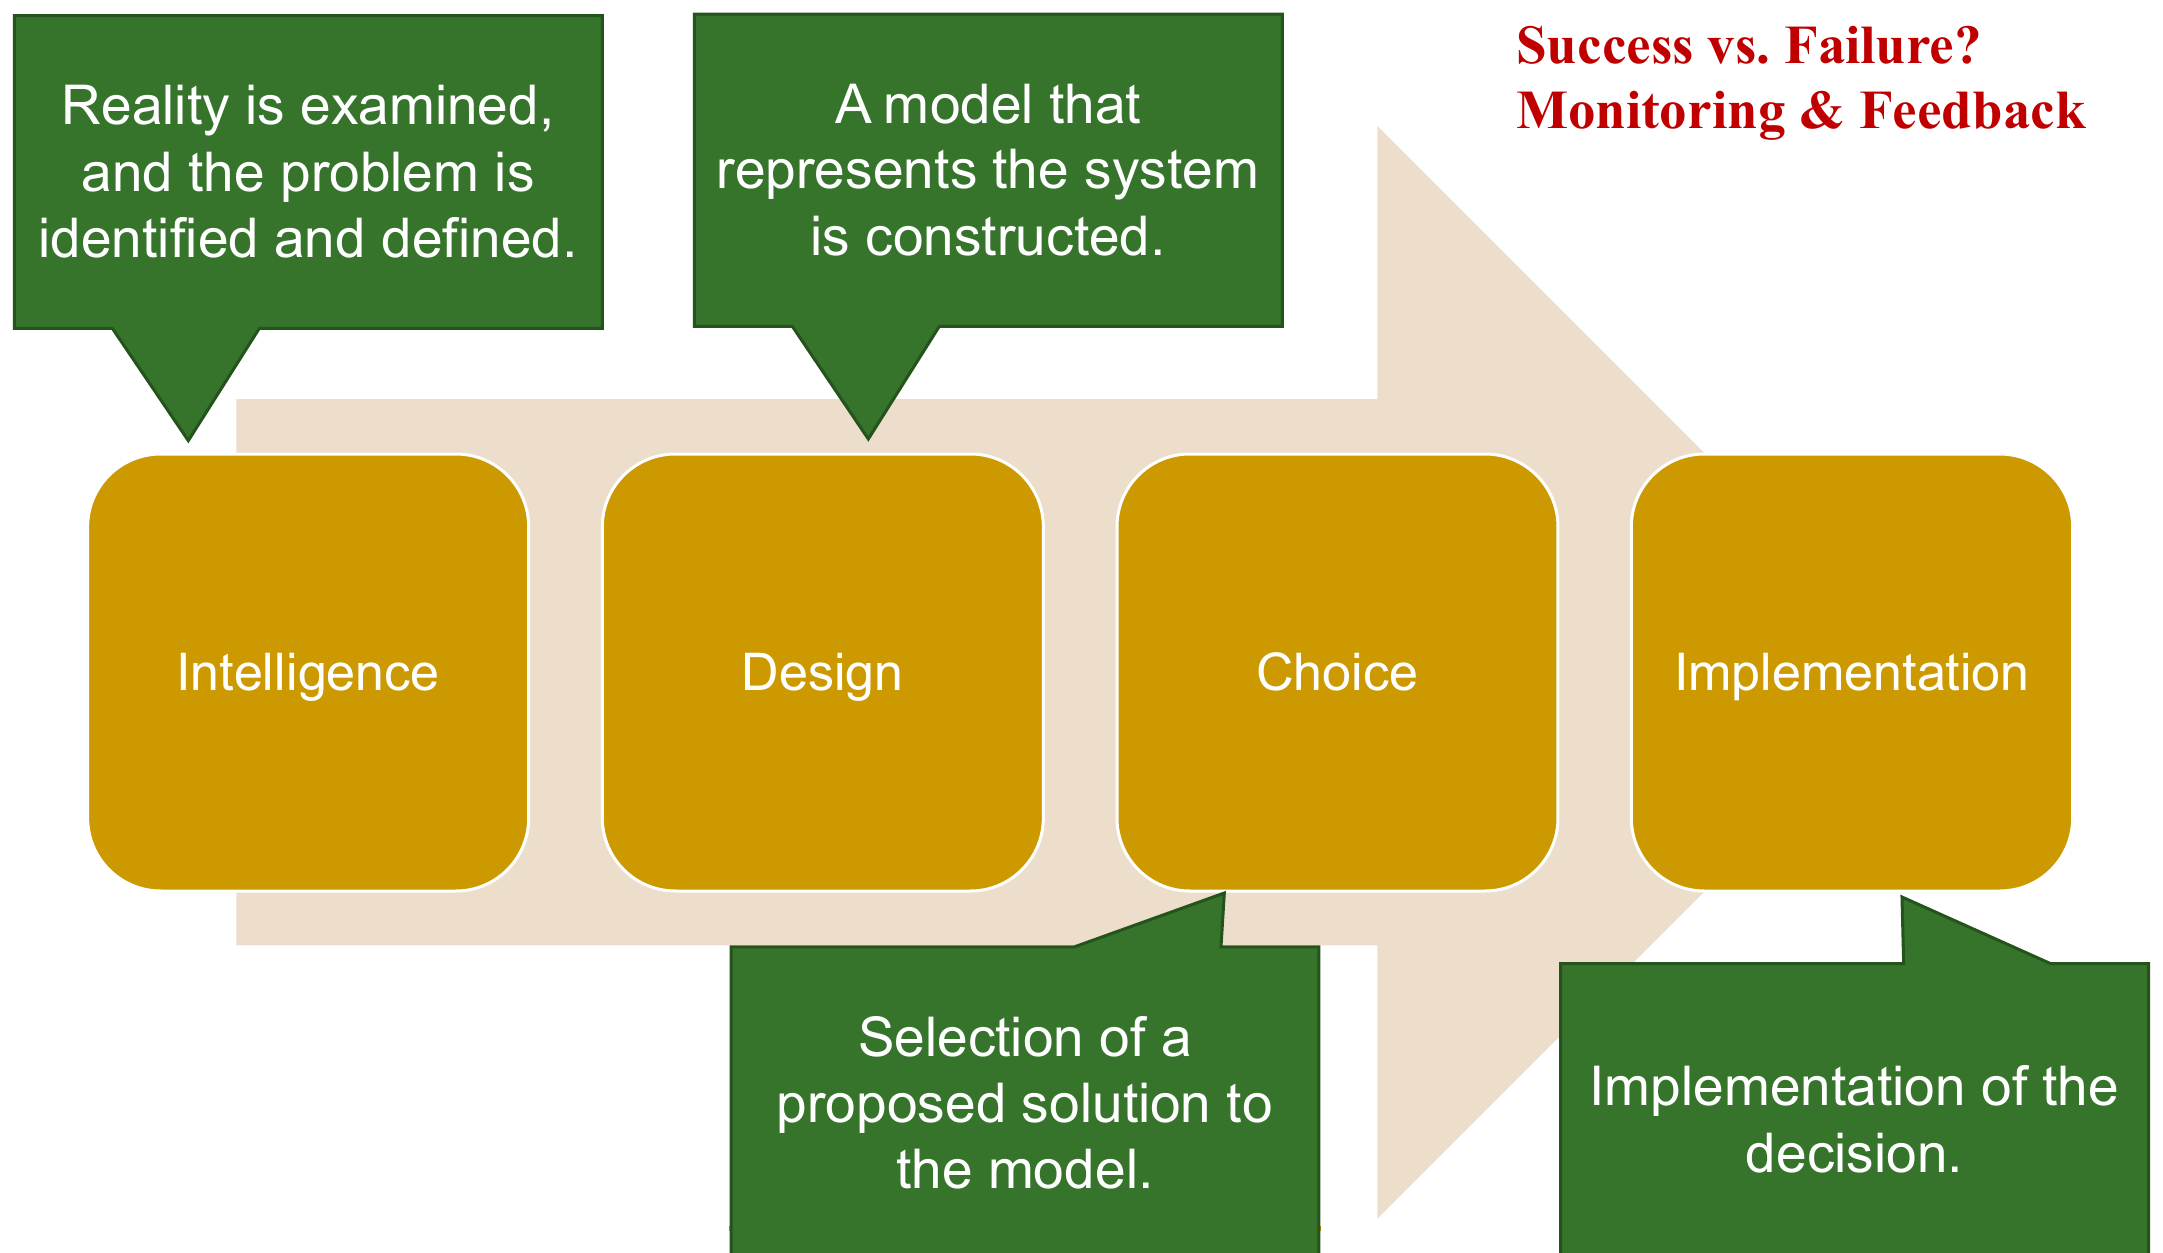
\includegraphics[width=0.85\textwidth]{slide/simon.png}
\caption{Bốn pha của quá trình ra quyết định theo Simon}
\label{fig:simon}
\end{figure}

\subsubsection{Đặc trưng và thành phần của DSS}
DSS hỗ trợ các vấn đề bán cấu trúc và phi cấu trúc, cho nhà quản lý ở mọi cấp. Một đặc trưng quan trọng là DSS nhắm tới hiệu quả của quyết định (effectiveness), không chỉ tới hiệu suất tính toán (efficiency). Con người vẫn là người kiểm soát, DSS chỉ cung cấp căn cứ. Hình~\ref{fig:dac_trung_dss} liệt kê đủ 14 đặc trưng của DSS theo Turban và Aronson~\cite{turban2005}.

\begin{figure}[!htbp]
\centering
% Vẽ lại từ hình trong slide (bản scan bị lỗi chữ)
\begin{tikzpicture}[
    dt/.style={align=center, text width=27mm, font=\scriptsize, inner sep=1pt},
    tia/.style={-{Stealth[length=1.8mm]}, thin}]
    \node[draw, thick, fill=gray!15, minimum width=16mm, minimum height=8mm, font=\small\bfseries] (dss) at (0,0) {DSS};
    \foreach \i/\chu in {
        1/{(1) Vấn đề bán cấu trúc và phi cấu trúc},
        2/{(2) Hỗ trợ nhà quản lý ở mọi cấp},
        3/{(3) Hỗ trợ cá nhân và nhóm},
        4/{(4) Quyết định phụ thuộc nhau hoặc tuần tự},
        5/{(5) Hỗ trợ đủ bốn pha ra quyết định},
        6/{(6) Nhiều phong cách và quy trình ra quyết định},
        7/{(7) Thích nghi và linh hoạt},
        8/{(8) Tương tác, dễ sử dụng},
        9/{(9) Hiệu quả, không chỉ hiệu suất},
        10/{(10) Con người kiểm soát máy},
        11/{(11) Người dùng cuối dễ tự phát triển},
        12/{(12) Mô hình hoá và phân tích},
        13/{(13) Truy cập dữ liệu},
        14/{(14) Độc lập, tích hợp hoặc trên nền Web}} {
        \pgfmathsetmacro{\goc}{90 - (\i - 1) * 360 / 14}
        \node[dt] (n\i) at ({5.9*cos(\goc)}, {3.9*sin(\goc)}) {\chu};
        \draw[tia] (dss) -- (n\i);
    }
\end{tikzpicture}
\caption{Mười bốn đặc trưng của DSS}
\label{fig:dac_trung_dss}
\end{figure}

Một DSS gồm bốn thành phần~\cite{turban2005}, như Hình~\ref{fig:thanh_phan_dss}:
\begin{itemize}
    \item \textbf{Quản lý dữ liệu:} lấy dữ liệu từ nguồn nội bộ, nguồn bên ngoài hoặc kho dữ liệu, rồi lưu vào cơ sở dữ liệu hỗ trợ quyết định.
    \item \textbf{Quản lý mô hình:} lưu và chạy các mô hình thống kê, tài chính, khoa học quản lý.
    \item \textbf{Quản lý tri thức:} cung cấp quy tắc nghiệp vụ và tri thức chuyên gia cho các thành phần khác.
    \item \textbf{Giao diện người dùng:} nơi người dùng tương tác với hệ thống.
\end{itemize}

\begin{figure}[!htbp]
\centering
\begin{tikzpicture}[
    tp/.style={draw, minimum width=30mm, minimum height=10mm, align=center, font=\small},
    noi/.style={{Stealth[length=2mm]}-{Stealth[length=2mm]}, thick}]
    \node[tp] (data) {Quản lý dữ liệu};
    \node[tp, right=14mm of data] (model) {Quản lý mô hình};
    \node[tp, below=8mm of $(data)!0.5!(model)$] (ui) {Giao diện người dùng};
    \node[tp, right=10mm of model, yshift=-9mm] (kb) {Quản lý tri thức};
    \node[tp, below=8mm of ui] (user) {Người ra quyết định};
    \draw[noi] (data) -- (model);
    \draw[noi] (data) -- (ui);
    \draw[noi] (model) -- (ui);
    \draw[noi] (kb) -- (ui);
    \draw[noi] (ui) -- (user);
    \node[tp, left=10mm of data] (src) {Kho dữ liệu,\\nguồn khác};
    \draw[-{Stealth[length=2.5mm]}, thick] (src) -- (data);
\end{tikzpicture}
\caption{Các thành phần của một DSS}
\label{fig:thanh_phan_dss}
\end{figure}

\subsubsection{Mô hình hoá và phân tích trong DSS}
Mô hình toán trong MSS có ba loại biến~\cite{turban2005}. Biến quyết định là những gì người ra quyết định chọn được. Biến không kiểm soát được, hay tham số, là các yếu tố môi trường như lãi suất hay giới hạn ngân sách. Biến kết quả đo mức độ đạt mục tiêu, ví dụ tổng lợi nhuận $Z$. Hình~\ref{fig:mo_hinh_toan} là ví dụ bài toán phối hợp sản phẩm. Bài toán tìm số lượng $X_1, X_2$ để cực đại $Z$ với các ràng buộc về tài nguyên, và được giải bằng quy hoạch tuyến tính hoặc quy hoạch nguyên.

\begin{figure}[!htbp]
\centering
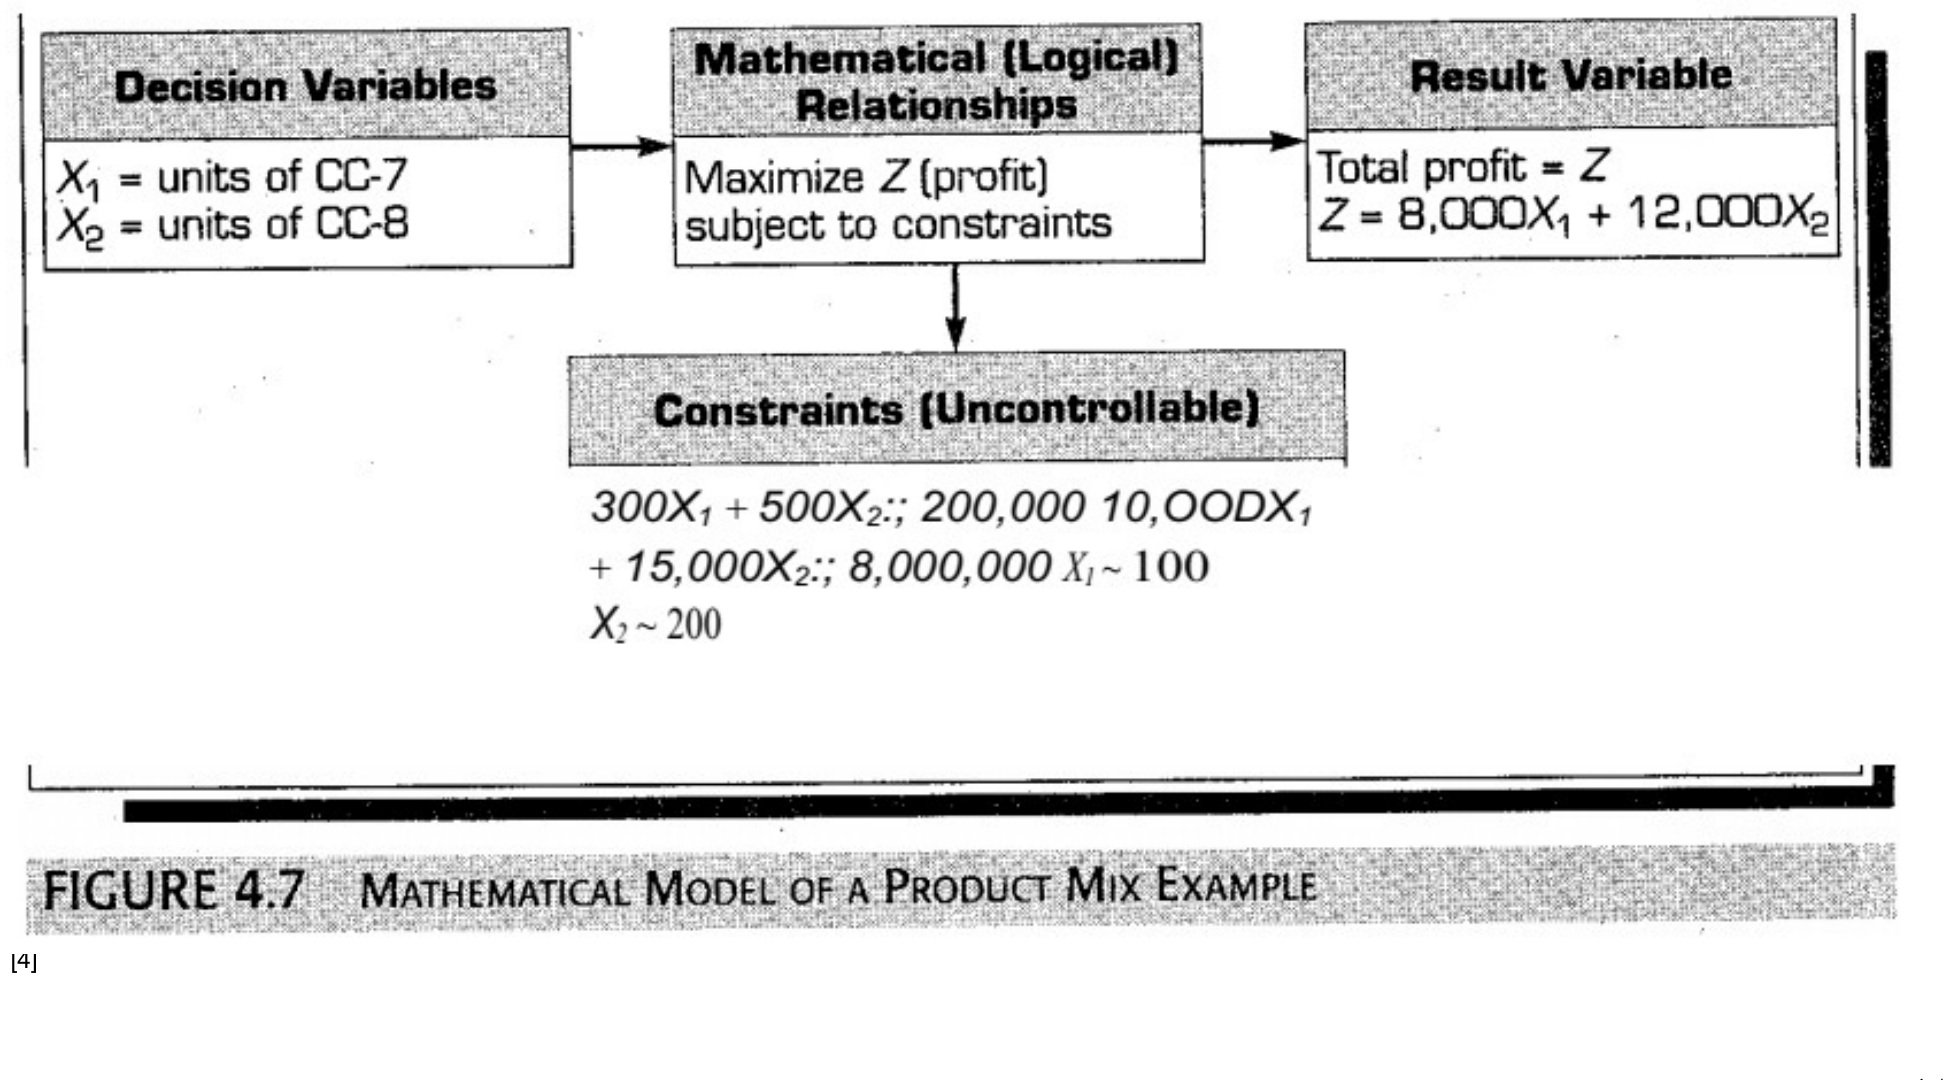
\includegraphics[width=0.85\textwidth]{slide/mo_hinh_toan_mss.png}
\caption{Cấu trúc mô hình toán của bài toán phối hợp sản phẩm}
\label{fig:mo_hinh_toan}
\end{figure}

Việc ra quyết định diễn ra trong ba điều kiện. Khi chắc chắn, người ra quyết định biết chính xác kết quả của mỗi phương án. Khi rủi ro, mỗi phương án có nhiều kết quả và biết được xác suất của từng kết quả. Lúc đó tiêu chí thường dùng là chọn phương án có giá trị kỳ vọng lớn nhất:
\begin{equation}
    EV(a) = \sum_{k} P(s_k)\, v(a, s_k)
\end{equation}
trong đó $P(s_k)$ là xác suất của tình huống $s_k$ và $v(a, s_k)$ là kết quả của phương án $a$ trong tình huống đó. Khi bất định, xác suất không ước lượng được, nên người ta dùng cách lạc quan (maximax) hoặc bi quan (maximin).

Sau khi có mô hình, DSS dùng bốn kiểu phân tích để người dùng khám phá phương án~\cite{turban2005}:
\begin{itemize}
    \item \textbf{What-if:} xem kết quả thay đổi thế nào khi đổi một biến hay một giả định.
    \item \textbf{Độ nhạy (sensitivity):} thay đổi một biến nhiều lần để xem kết quả nhạy với biến đó đến đâu.
    \item \textbf{Tìm mục tiêu (goal seeking):} tìm giá trị đầu vào cần có để đạt một mục tiêu cho trước.
    \item \textbf{Tối ưu hoá (optimization):} tìm giá trị tốt nhất của biến mục tiêu bằng cách thay đổi các biến khác.
\end{itemize}

\subsection{Phương pháp khai phá dữ liệu}
Khai phá dữ liệu (data mining) là quá trình tìm ra các mẫu và tri thức có ích từ lượng dữ liệu lớn~\cite{han2011}. Nó là một bước trong quy trình khám phá tri thức (KDD) ở Hình~\ref{fig:kdd}: làm sạch và tích hợp, đưa vào kho, chọn và biến đổi, khai phá, rồi đánh giá và trình bày. Các bài toán chính gồm phân lớp, gom cụm, luật kết hợp và phát hiện ngoại lai.

\begin{figure}[!htbp]
\centering
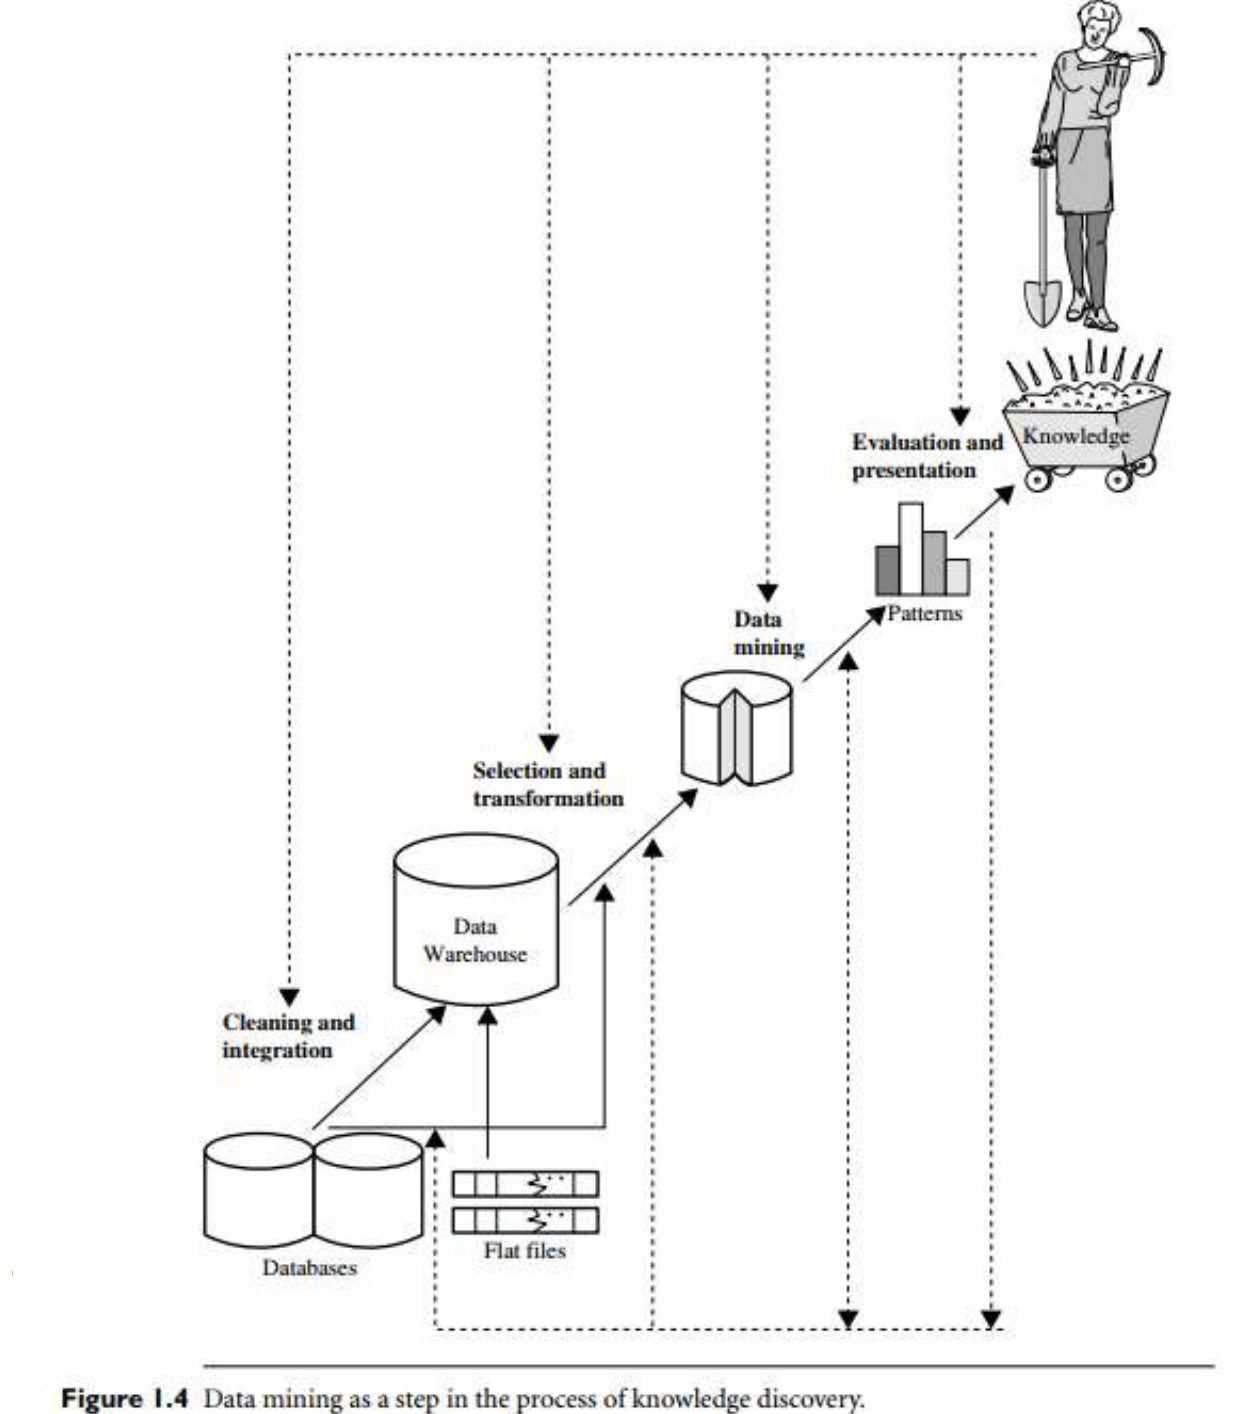
\includegraphics[width=0.6\textwidth]{slide/kdd.png}
\caption{Khai phá dữ liệu là một bước trong quy trình khám phá tri thức}
\label{fig:kdd}
\end{figure}

\subsubsection{Phân lớp và đánh giá mô hình}
Phân lớp (classification) là tìm một mô hình mô tả và phân biệt các lớp dữ liệu. Quá trình có hai bước~\cite{han2011}, như Hình~\ref{fig:phan_lop}. Ở bước học, mô hình được xây dựng từ tập huấn luyện đã có nhãn. Ở bước phân lớp, mô hình được dùng để dự đoán nhãn cho dữ liệu mới. Trước khi dùng, mô hình được kiểm tra trên một tập dữ liệu có nhãn khác để đo độ chính xác.

\begin{figure}[!htbp]
\centering
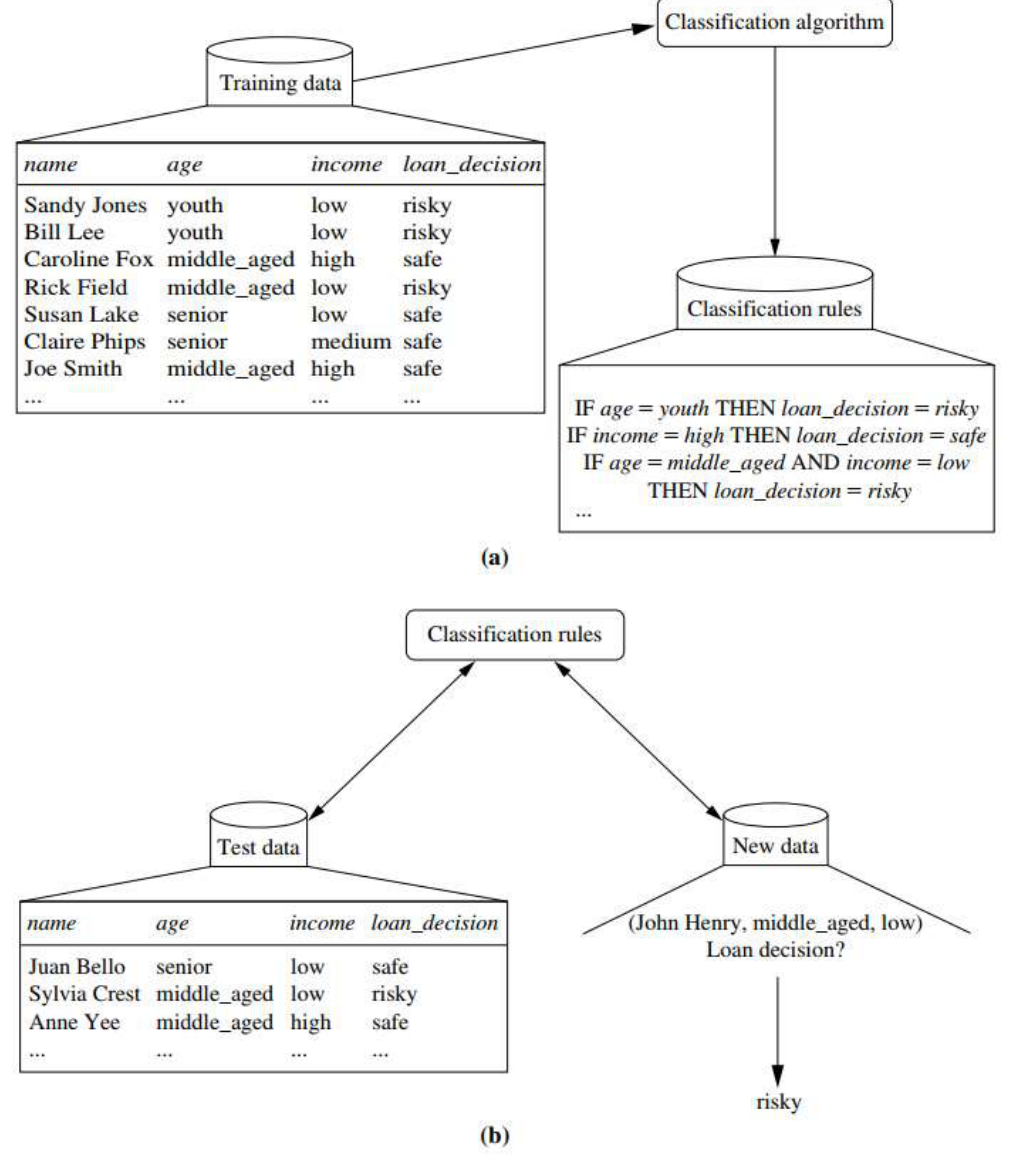
\includegraphics[width=0.62\textwidth]{slide/phan_lop_hai_buoc.png}
\caption{Hai bước của bài toán phân lớp: (a) bước học, (b) bước phân lớp}
\label{fig:phan_lop}
\end{figure}

Kết quả phân lớp hai lớp được tóm tắt bằng ma trận nhầm lẫn ở Bảng~\ref{tab:ma_tran_nham_lan}.

\begin{table}[!htbp]
\centering
\caption{Ma trận nhầm lẫn cho bài toán hai lớp}
\label{tab:ma_tran_nham_lan}
\begin{tabular}{llcc}
\toprule
 & & \multicolumn{2}{c}{\textbf{Dự đoán}} \\
 & & Dương & Âm \\
\midrule
\multirow{2}{*}{\textbf{Thực tế}} & Dương ($P$) & TP & FN \\
 & Âm ($N$) & FP & TN \\
\bottomrule
\end{tabular}
\end{table}

Từ ma trận này tính được các chỉ số đánh giá~\cite{han2011}:
\begin{align}
    \text{Accuracy} &= \frac{TP + TN}{P + N}, &
    \text{Error rate} &= \frac{FP + FN}{P + N}, \\
    \text{Recall} &= \frac{TP}{P}, &
    \text{Specificity} &= \frac{TN}{N}, \\
    \text{Precision} &= \frac{TP}{TP + FP}, &
    F_1 &= \frac{2 \times \text{Precision} \times \text{Recall}}{\text{Precision} + \text{Recall}}.
\end{align}
Accuracy dễ bị đánh lừa khi một lớp chiếm đa số. Khi đó precision, recall và specificity cho biết rõ hơn mô hình sai ở lớp nào.

\subsubsection{Cây quyết định}
Cây quyết định chia dữ liệu dần theo từng thuộc tính. Mỗi nút trong kiểm tra một thuộc tính, mỗi nhánh là một kết quả kiểm tra, và mỗi lá là một nhãn lớp. Các thuật toán phổ biến là ID3, C4.5 và CART~\cite{han2011}. Mỗi đường đi từ gốc tới lá đọc được thành một luật IF--THEN, nên cây dễ giải thích cho người không chuyên.

Tại mỗi nút, thuật toán chọn thuộc tính chia tốt nhất. ID3 dùng độ lợi thông tin (information gain):
\begin{equation}
    Info(D) = -\sum_{i=1}^{m} p_i \log_2 p_i, \qquad
    Gain(A) = Info(D) - \sum_{j=1}^{v} \frac{|D_j|}{|D|}\, Info(D_j)
\end{equation}
trong đó $p_i$ là tỷ lệ bản ghi thuộc lớp $C_i$, và thuộc tính $A$ chia $D$ thành $v$ tập con $D_j$. CART dùng chỉ số Gini, công thức này ngoài nội dung môn học:
\begin{equation}
    Gini(D) = 1 - \sum_{i=1}^{m} p_i^2
\end{equation}
Gini bằng 0 khi nút chỉ có một lớp. Thuộc tính được chọn là thuộc tính làm Gini trung bình có trọng số của các nút con giảm nhiều nhất.

Hình~\ref{fig:cay_churn} là một ví dụ cây Gini cho bài toán churn trong tài liệu môn học~\cite{tlmh}. Cây chia nhân viên theo thời gian làm việc và mức lương, mỗi lá ghi nhãn Quit (rời đi) hoặc Stayed (ở lại). Trên mỗi nút có chỉ số gini, số mẫu và số mẫu của từng lớp.

\begin{figure}[!htbp]
\centering
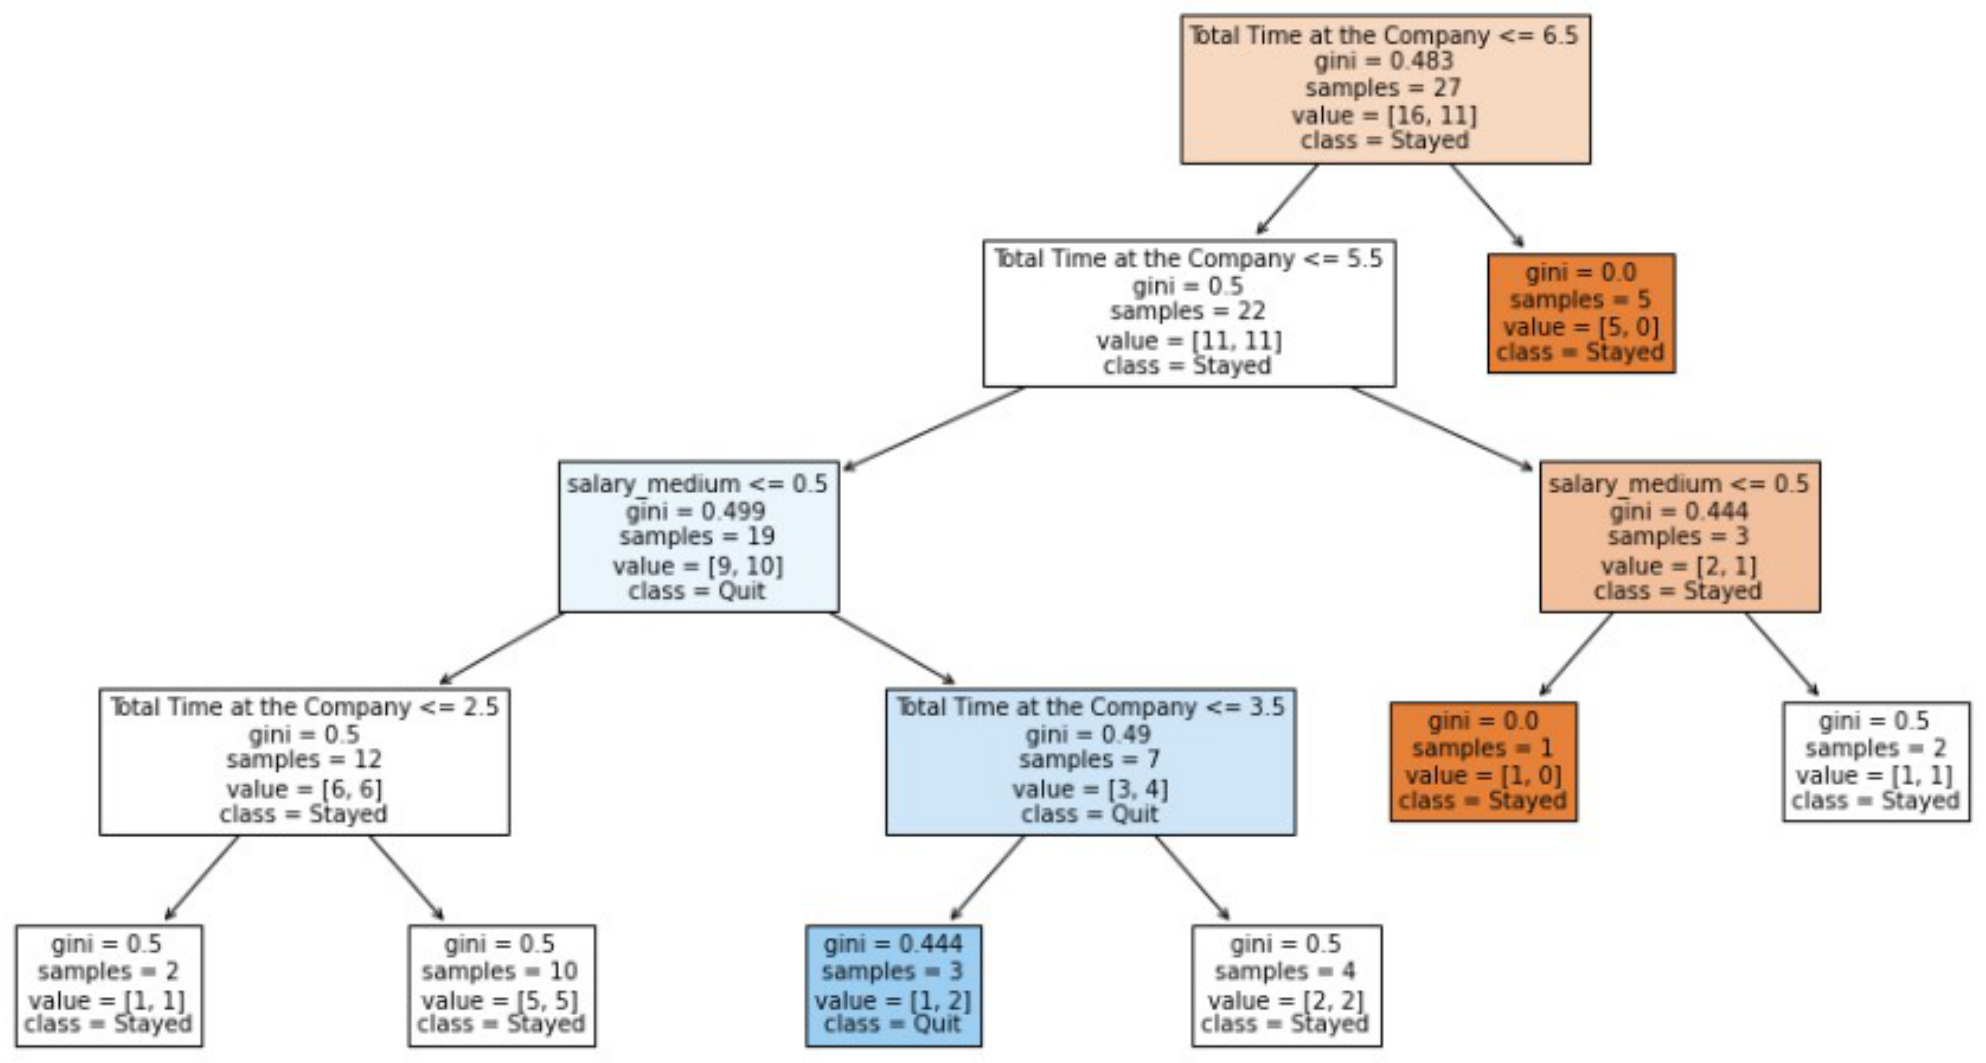
\includegraphics[width=0.9\textwidth]{slide/cay_churn.png}
\caption{Ví dụ cây quyết định Gini cho bài toán churn}
\label{fig:cay_churn}
\end{figure}

\subsubsection{Bộ phân lớp Naive Bayes}
Naive Bayes dựa trên định lý Bayes~\cite{han2011}:
\begin{equation}
    P(C_i \mid X) = \frac{P(X \mid C_i)\, P(C_i)}{P(X)}
\end{equation}
trong đó $X$ là một bản ghi và $C_i$ là một lớp. Mô hình gán $X$ vào lớp có $P(X \mid C_i)P(C_i)$ lớn nhất. Để tính $P(X \mid C_i)$ cho đơn giản, mô hình giả định các thuộc tính độc lập với nhau khi đã biết lớp:
\begin{equation}
    P(X \mid C_i) = \prod_{k=1}^{n} P(x_k \mid C_i)
\end{equation}
Giả định này hiếm khi đúng hoàn toàn trong thực tế. Dù vậy, mô hình vẫn thường xếp hạng tốt và cho ra trực tiếp xác suất của từng lớp. Khi một giá trị thuộc tính chưa từng xuất hiện trong một lớp, xác suất bằng 0 sẽ làm cả tích bằng 0. Cách xử lý thường dùng là làm trơn Laplace, cộng thêm một số nhỏ vào mỗi lần đếm. Kỹ thuật này ngoài nội dung môn học.

\subsubsection{Mạng nơ-ron, gom cụm và luật kết hợp}
Mô hình phân lớp cũng có thể biểu diễn bằng mạng nơ-ron~\cite{han2011}. Mạng nhiều tầng (Multi-Layer Perceptron, MLP) gồm tầng đầu vào, một hay nhiều tầng ẩn và tầng đầu ra. Mạng được huấn luyện bằng lan truyền ngược (backpropagation). Phần MLP và lan truyền ngược ngoài nội dung môn học.

Gom cụm k-means chia dữ liệu thành $k$ cụm~\cite{han2011}. Thuật toán chọn $k$ tâm ban đầu, gán mỗi điểm vào cụm có tâm gần nhất, cập nhật tâm bằng trung bình của cụm, rồi lặp lại đến khi ổn định. Số cụm $k$ thường được chọn bằng phương pháp khuỷu tay (elbow) dựa trên tổng bình phương khoảng cách trong cụm, hoặc bằng hệ số Silhouette.

Luật kết hợp tìm các mặt hàng hay được mua cùng nhau, ví dụ bằng thuật toán Apriori. Một luật $A \Rightarrow B$ được đánh giá bằng ba chỉ số:
\begin{equation}
    \text{support} = P(A \cup B), \qquad
    \text{confidence} = \frac{P(A \cup B)}{P(A)}, \qquad
    \text{lift} = \frac{P(A \cup B)}{P(A)\,P(B)}
\end{equation}
Lift lớn hơn 1 nghĩa là $A$ và $B$ xuất hiện cùng nhau nhiều hơn mức ngẫu nhiên.
